
\chapter{Data Curation}
\label{ch:data}

%This chapter covers data aspects of the challenge.

\section{Data Sets}

\subsection{prompts\_train.csv}

The prompts\_train.csv consists of 4 columns:

\begin{itemize}
	\item \textbf{prompt\_id:} The unique ID of the prompt which links to the summaries file.
	\item \textbf{prompt\_question:} The specific question the students are asked to answer.%respond to.
	\item \textbf{prompt\_title:} A short-hand title for the prompt.
	\item \textbf{prompt\_text:} The full prompt text.
\end{itemize}

This dataset only contains 4 entries, since there are only 4 different reference texts.

\subsection{summaries\_train.csv}

The summaries\_train.csv consists of 5 columns:

\begin{itemize}
	\item \textbf{student\_id:} The unique ID of the student writer.
	\item \textbf{prompt\_id:} The unique ID of the prompt which links to the prompt file. 
	\item \textbf{text:} The full text of the student's summary.
	\item \textbf{content:} The content score for the summary. The first target.
	\item \textbf{wording:} The wording score for the summary. The second target.

\end{itemize}

This dataset contains over 7'000 entries with varying content- and wording scores.

%Further details regarding the data can be found in the section \ref{sec:data-quality-assessment}.

\section{Data Quality Assessment} \label{sec:data-quality-assessment}

%This section describes on how the data quality assessment was conducted.
The given data was of high quality because it was already cleaned up by the hosts of the competition, thus there were no empty or invalid entries. Data augmentation, using back-translation and paraphrasing techniques, did not work for this project since it was impossible to predict valid and logical content and wording score for the augmented student summaries.
The most interesting features for predicting our target variables were the prompt texts, student summaries, and prompt questions.
The IDs were used to merge the prompts and summaries datasets. This was done to just have one final training dataset.

\subsection{Data Overview and Plots}

%First, the distribution of the wording and content scores was analyzed.
The distribution of the content score, as seen in Figure \ref{fig:content-score}, is evenly right-skewed while the distribution of the wording score, as seen in Figure \ref{fig:wording-score}, shows spikes in certain score ranges. The cause of those spikes occuring has not been determined, as no clear similarities between student summaries within that scoring range were found.\\

\begin{figure}[H]
\begin{center}
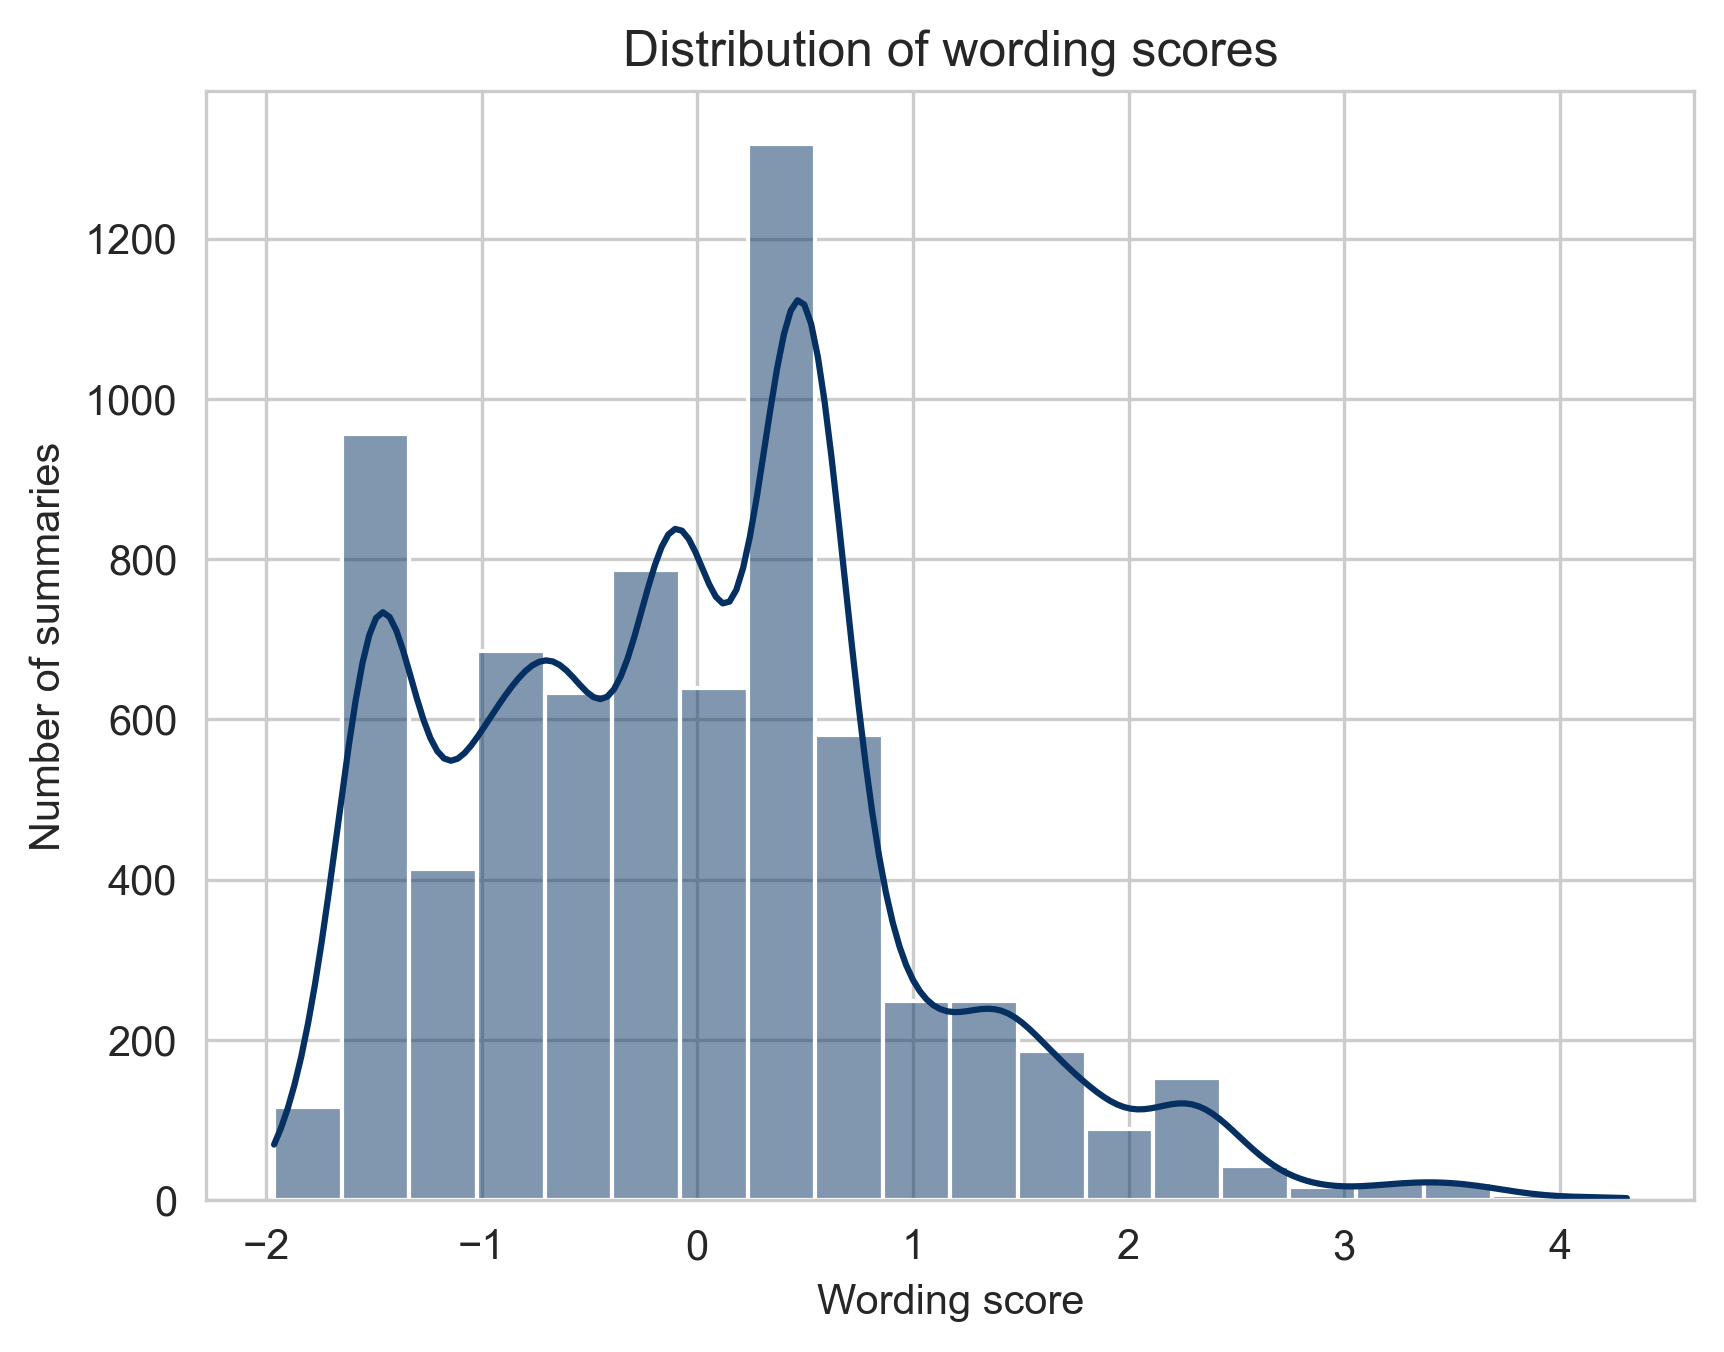
\includegraphics[width=80mm,scale=0.75]{img/wording_score.png}
\end{center}
\caption[Distribution of Wording scores]{Distribution of the training set wording scores. Two large spikes can be seen indicating similar scores for many student summaries}
%TODO Update Image with Question input for transfomer
\label{fig:wording-score}
\end{figure}

\begin{figure}[H]
\begin{center}
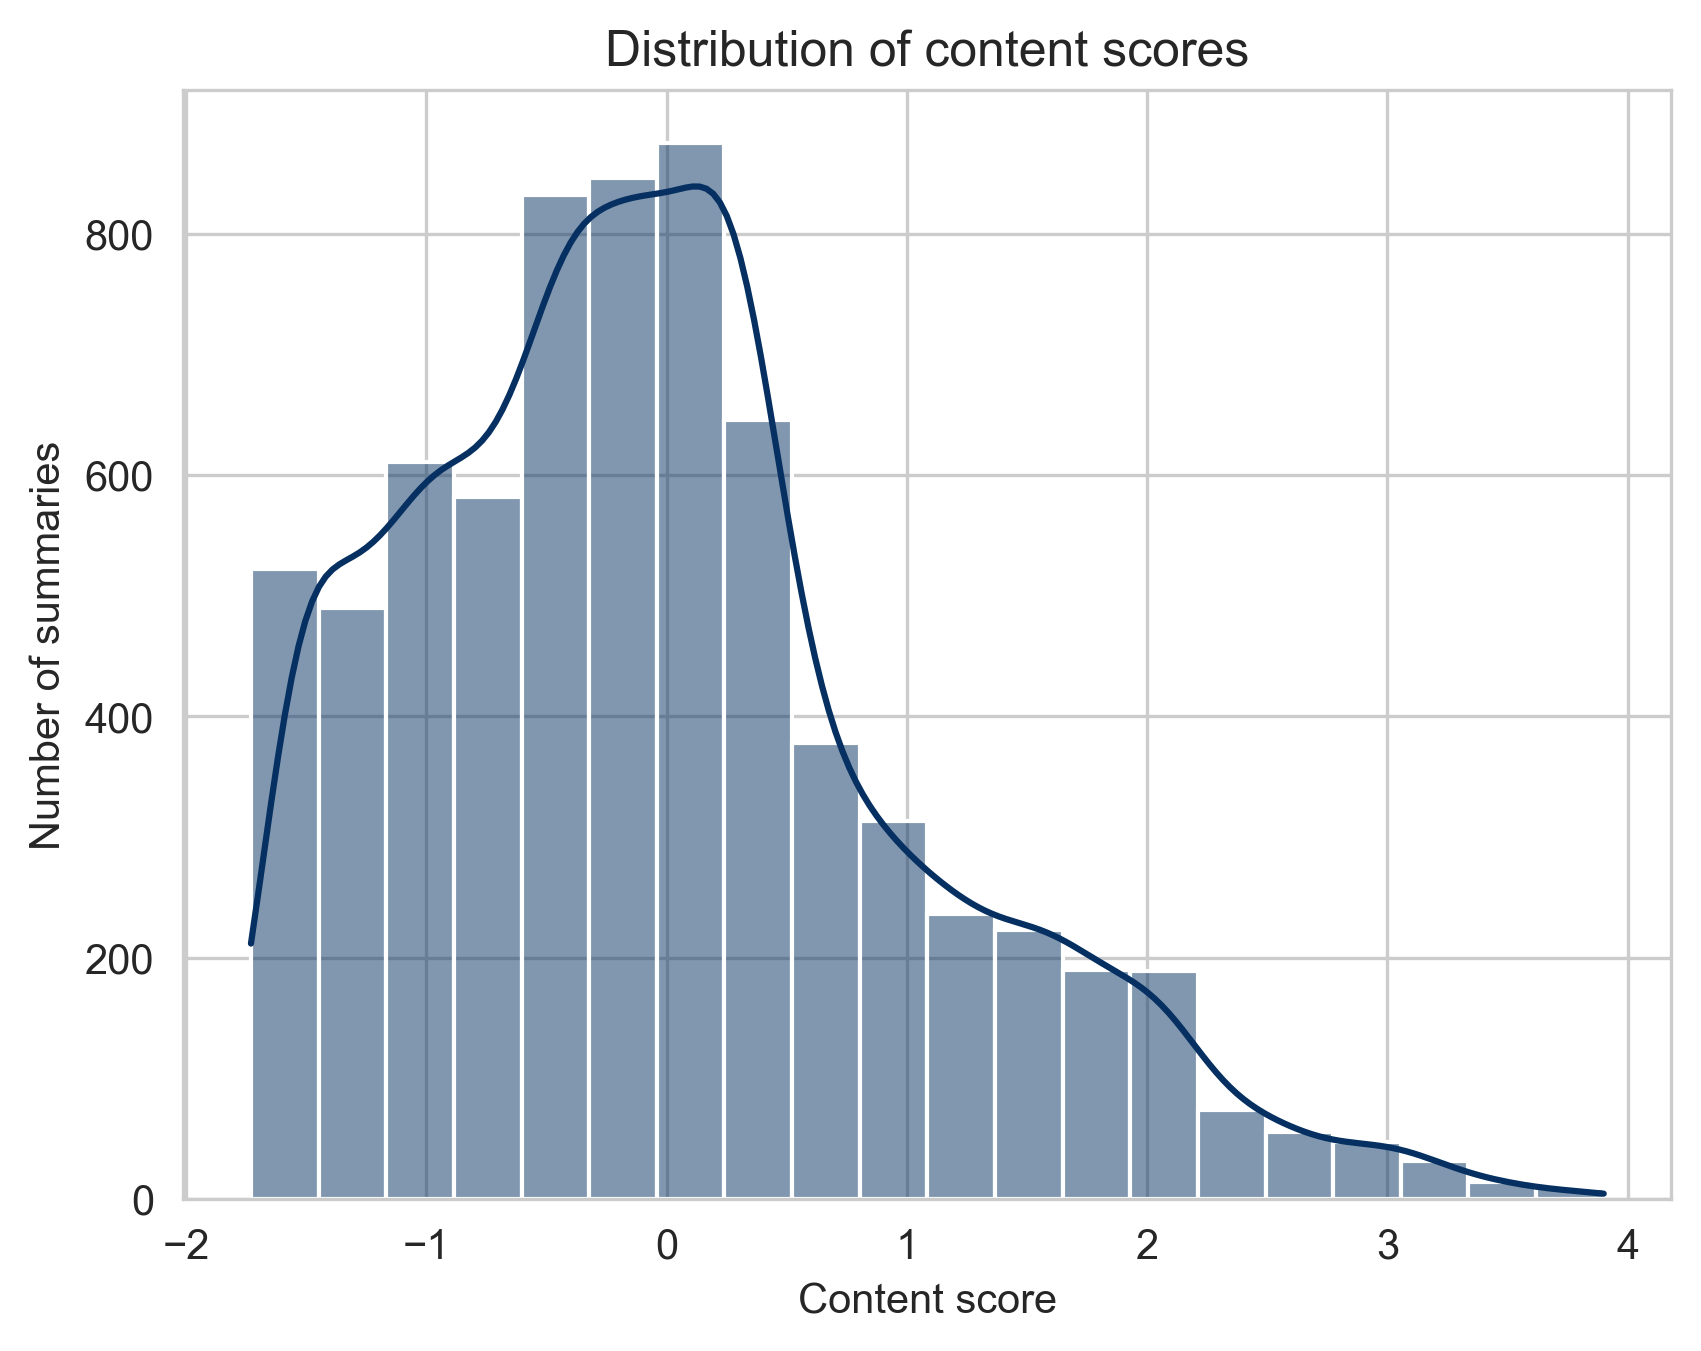
\includegraphics[width=80mm,scale=0.75]{img/content_score.png}
\end{center}
\caption[Distribution of Content scores]{Distribution of the training set content scores. The content score seems to be more evenly distributed than the wording score.}
\label{fig:content-score}
\end{figure}%

\noindent Due to the fact, that most wording and content scores are under 1, it has been assumed
that both scores were graded very strictly by the experts. Consequently, the team also assumed that any machine learning models would give scores in similar ranges, due to those models being trained on those ranges.\\

\noindent It was also assumed, that the test set on Kaggle has a similar distribution, though this could not be verified as the team did not have access to the final test data.\\

\pagebreak
\noindent Additionally, the number of student summaries for every reference topic has been analyzed as well. As seen in Figure \ref{fig:num-of-texts-per-prompt}, student summaries about the topic "The Third Wave" are underrepresented in this dataset, however this did not matter as the final test set contained hundreds of different topics.\\

\begin{figure}[H]
\begin{center}
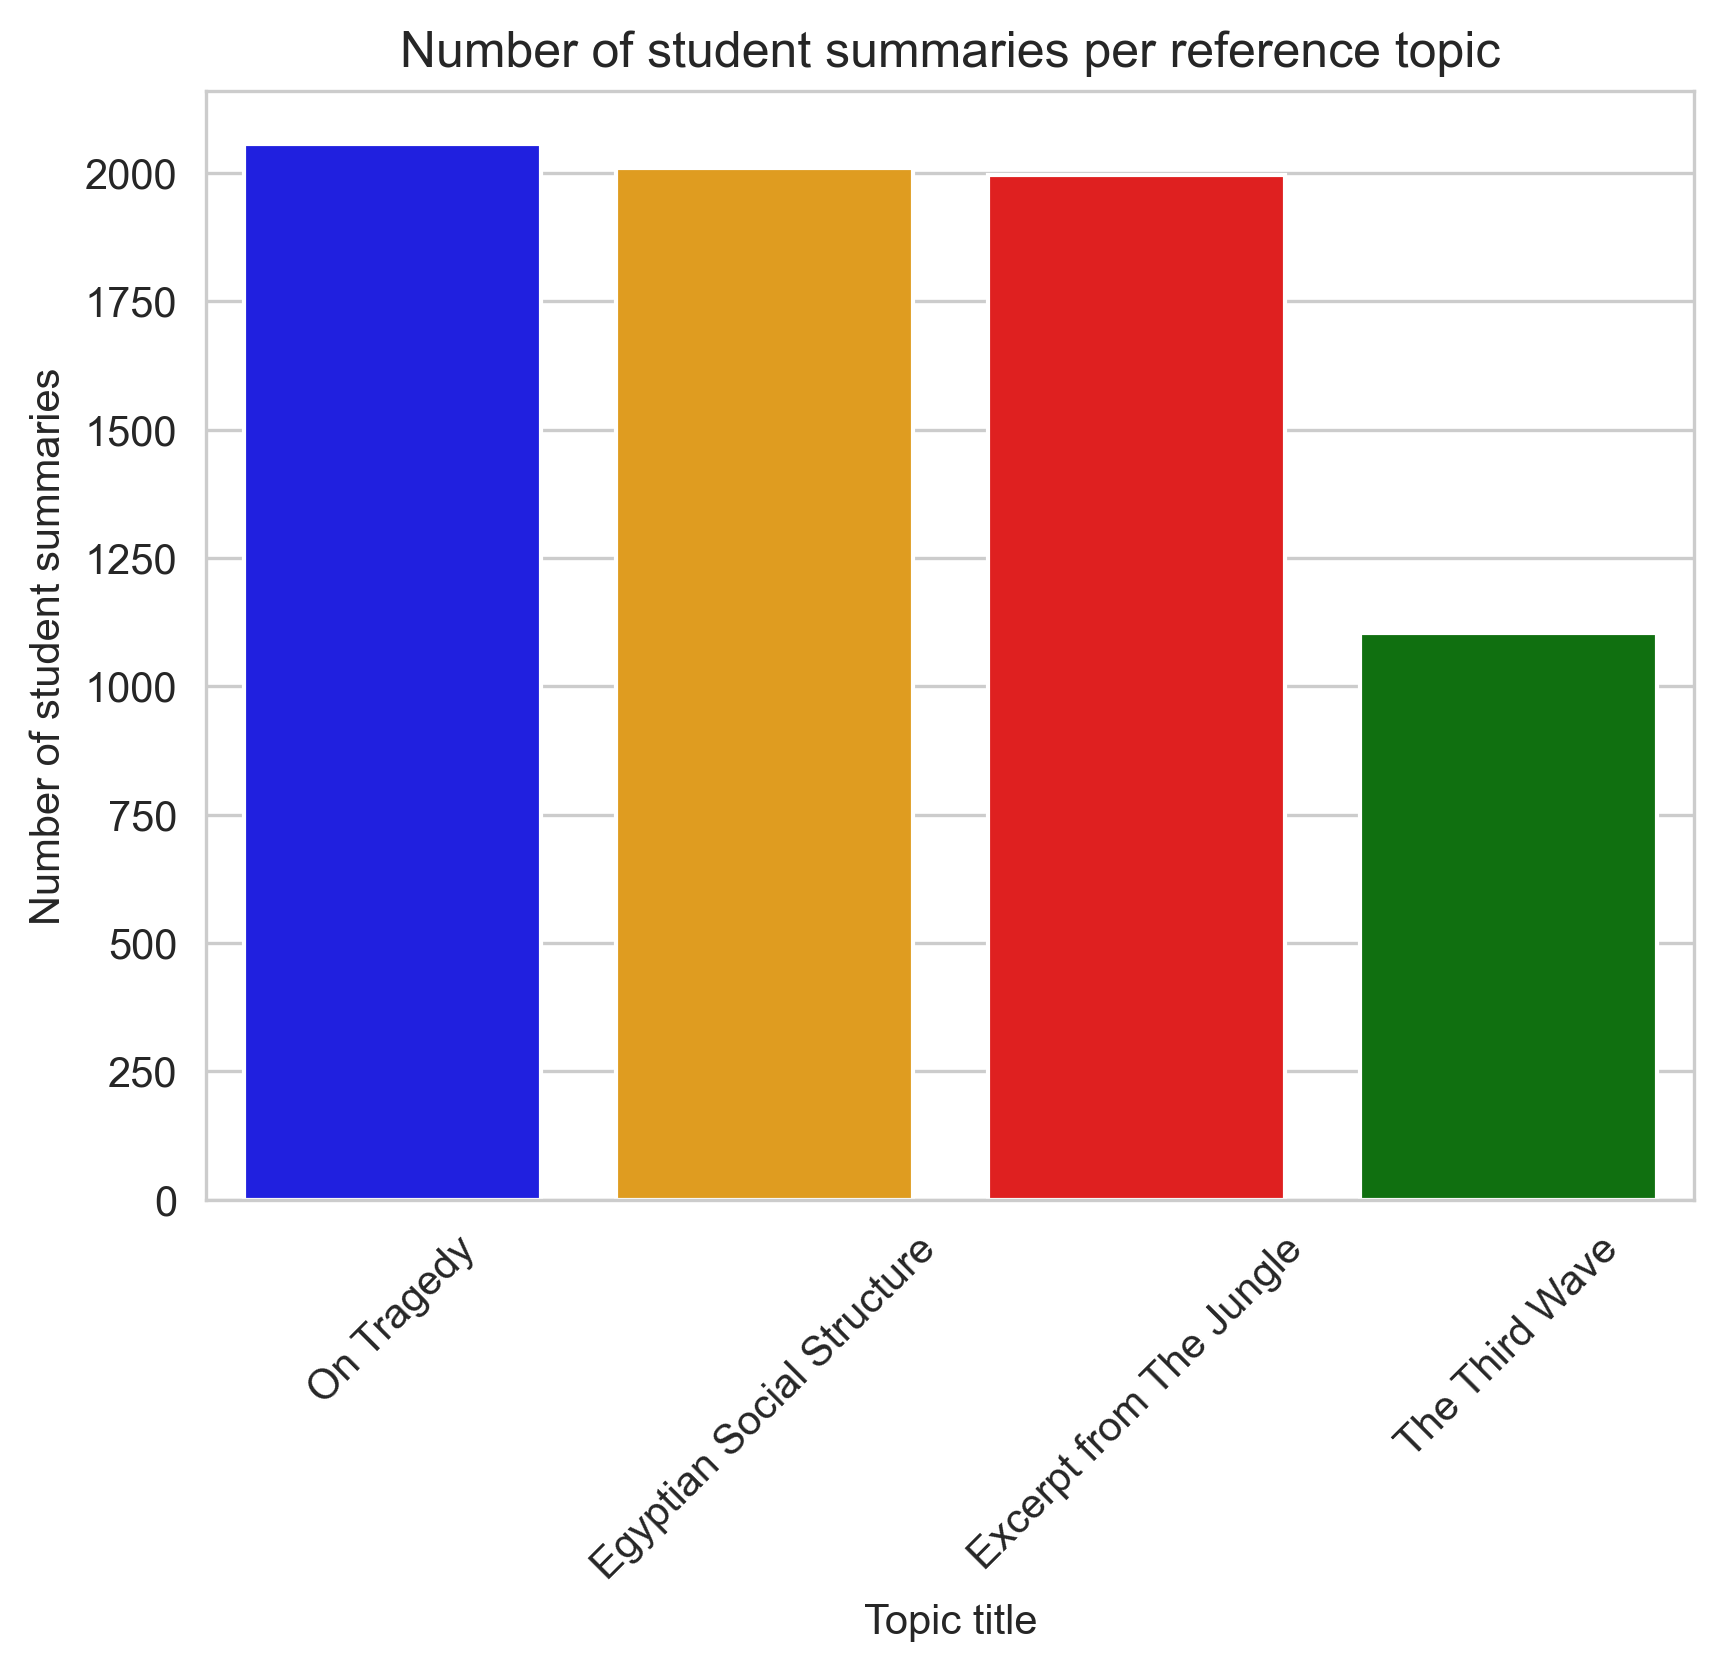
\includegraphics[width=80mm,scale=0.75]{img/number_of_texts_per_prompt.png}
\end{center}
\caption[Number of student summaries per topic]{The topic "Third Wave" is underrepresented in the training dataset.}
\label{fig:num-of-texts-per-prompt}
\end{figure}
\pagebreak
\noindent The length ratio between student summaries and reference texts in relation to both scores were plotted as well. For some reference text topics, like 'On Tragedy' or 'Egyptian Social Structure', there were certain instances, where the length of the summary turned out to be longer than the reference text itself, despite the objective of this task being summarization.
%We believe this to be an oversight by the experts.
See Figure \ref{fig:wording-ratio} and Figure \ref{fig:content-ratio} for the mentioned plots.\\


\begin{figure}[H]
\begin{center}
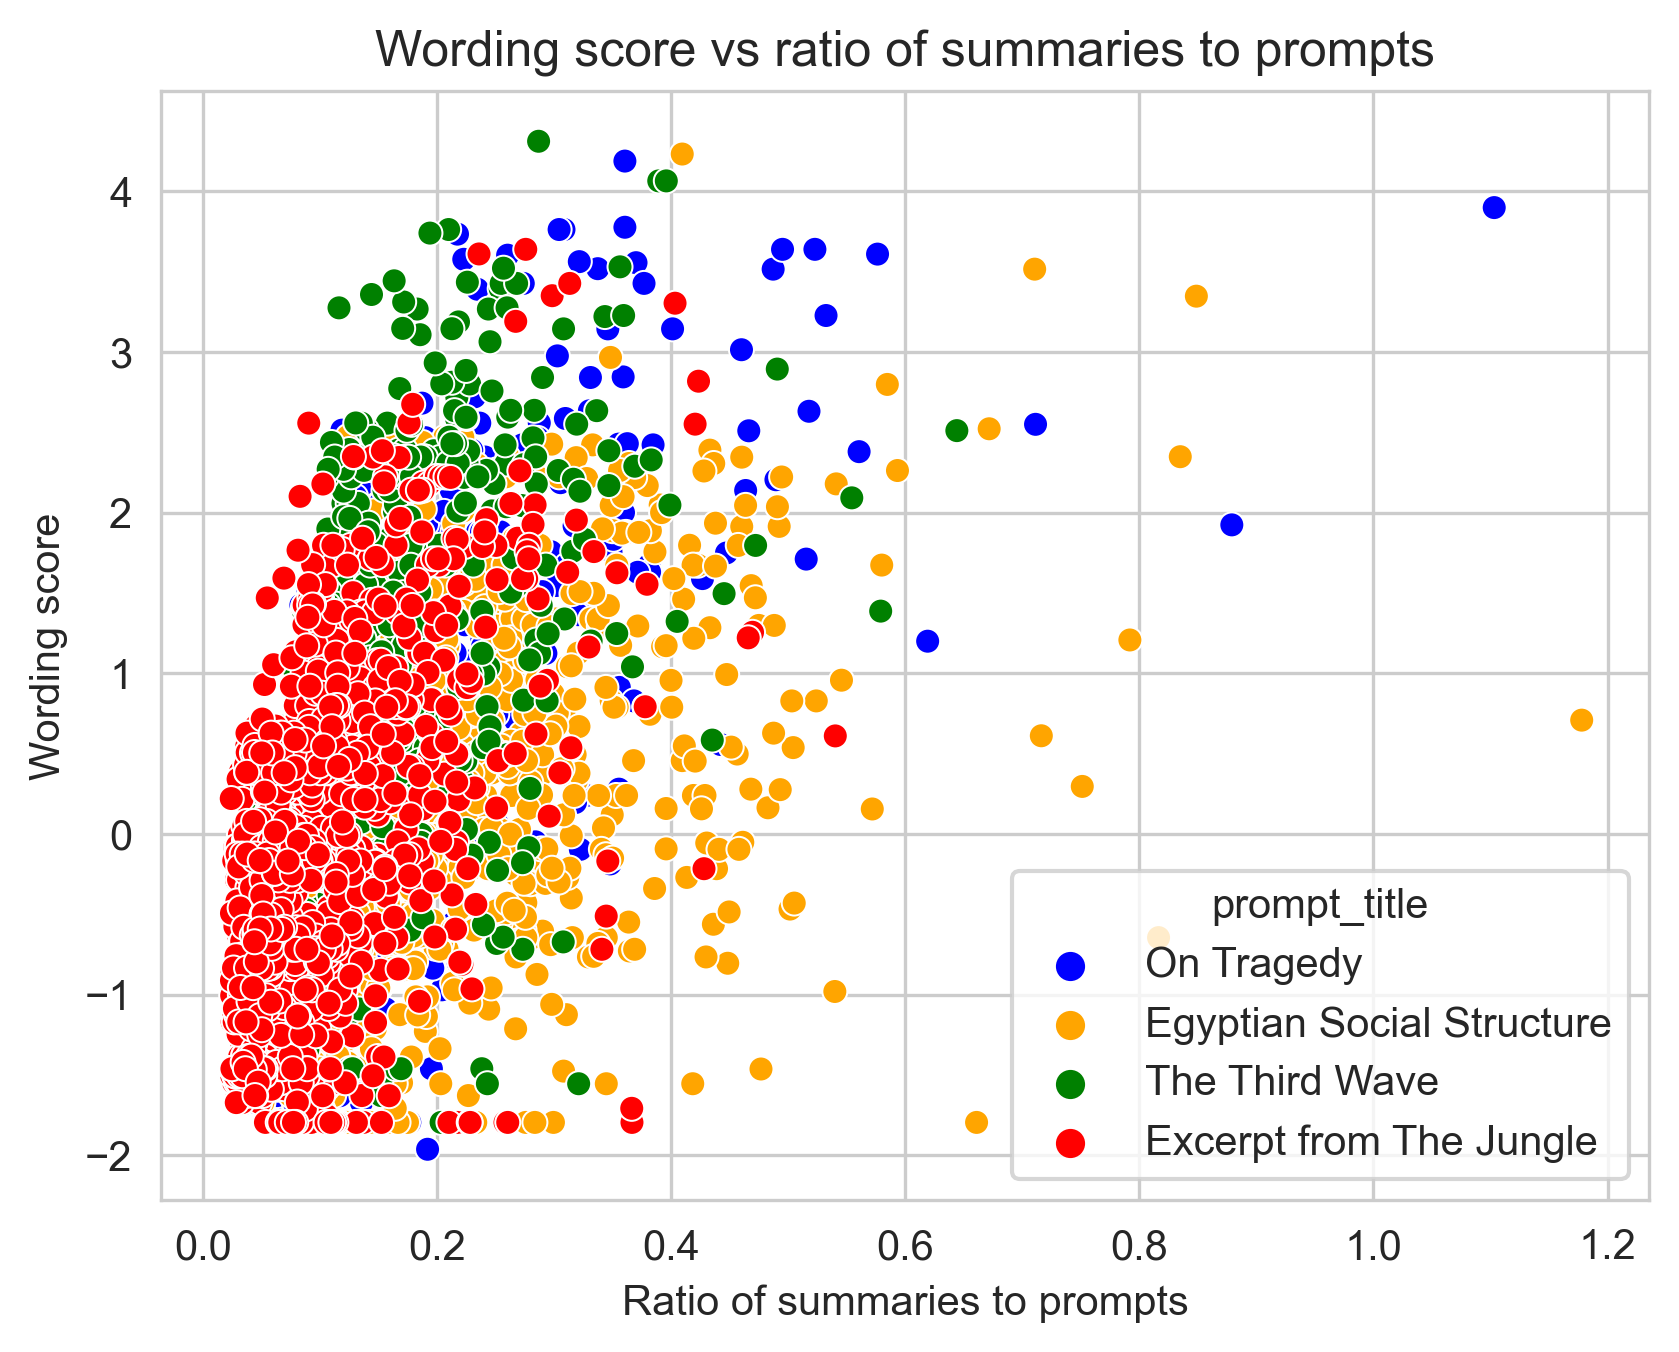
\includegraphics[width=80mm,scale=0.75]{img/wording_ratio_summaries_to_prompts.png}
\end{center}
\caption{Wording scores in relation to the length ratio of student summaries and reference texts.}
\label{fig:wording-ratio}
\end{figure}


\begin{figure}[H]
\begin{center}
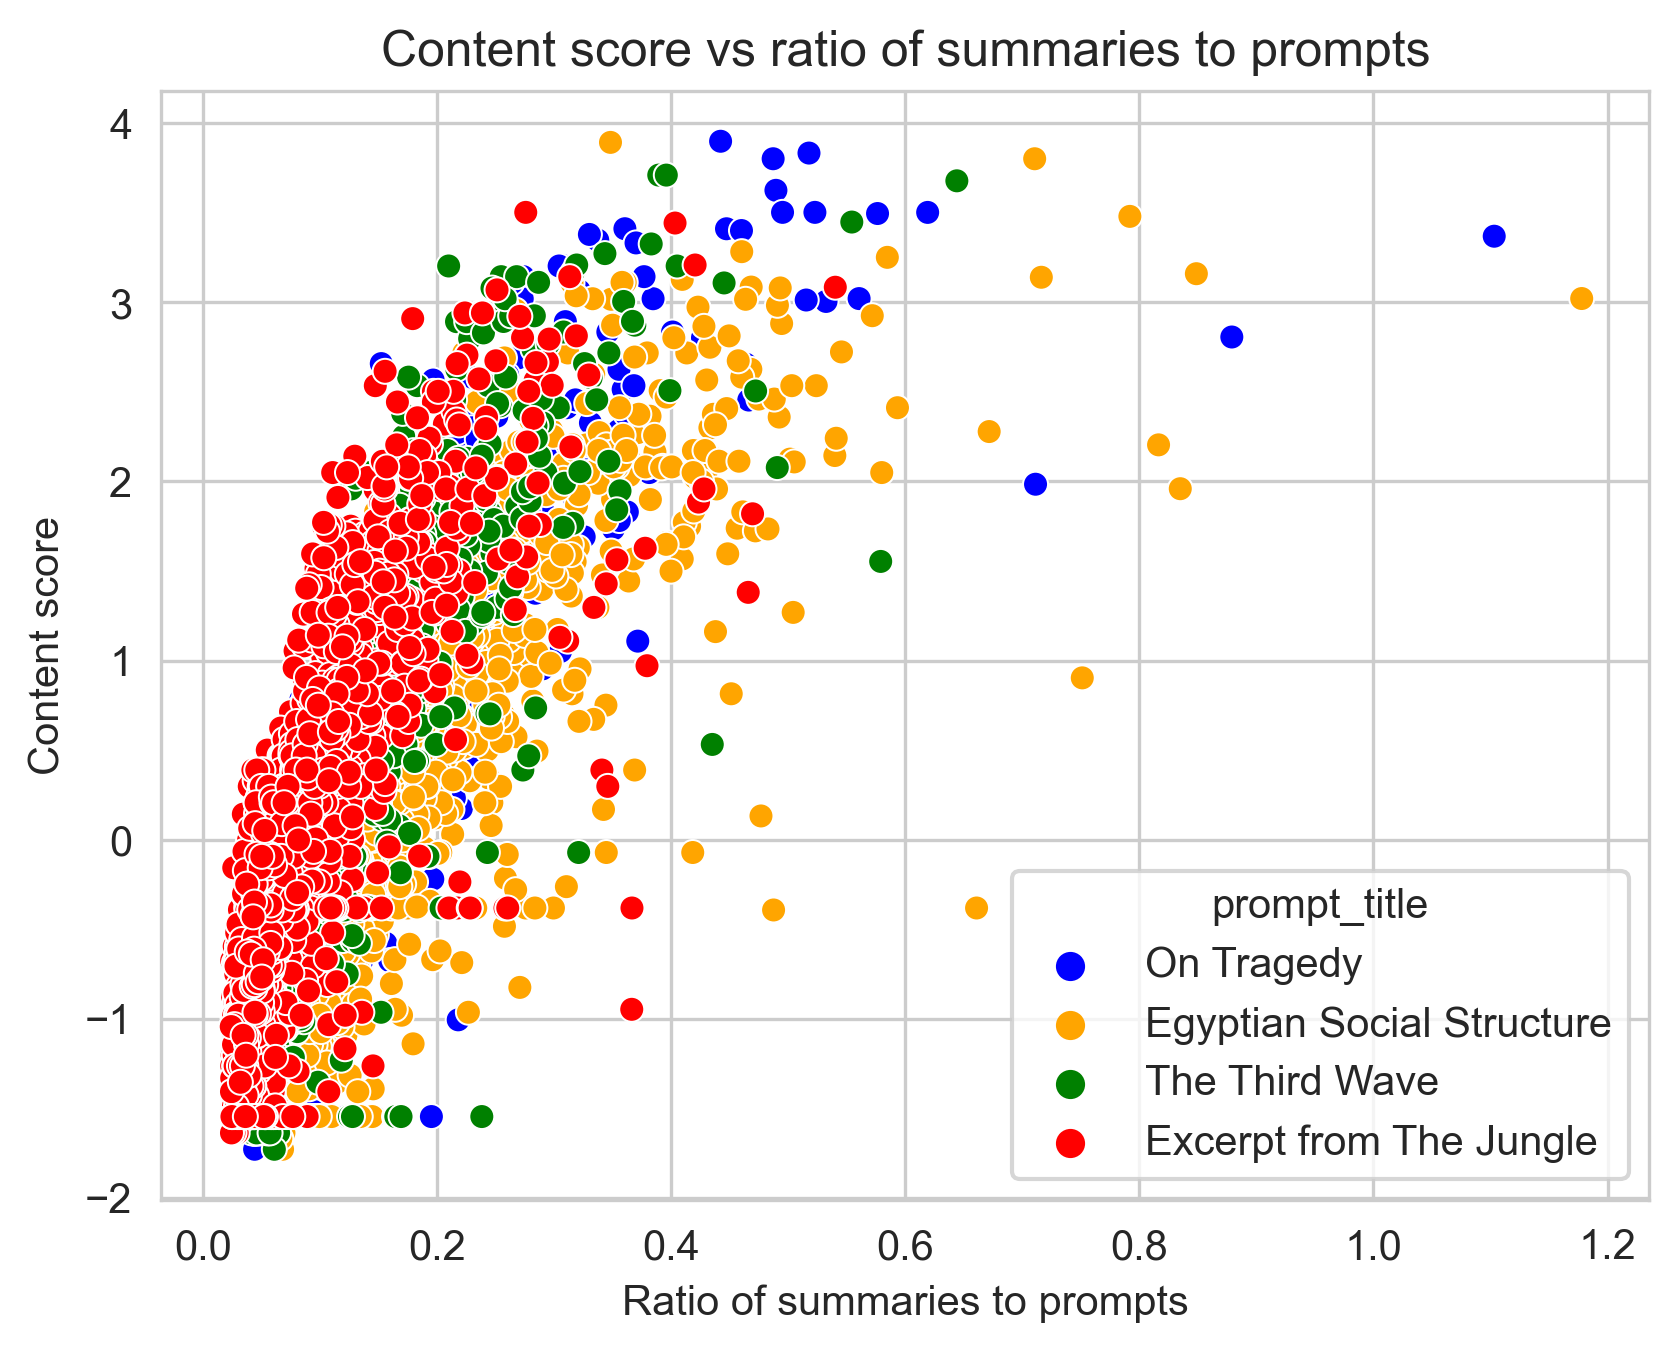
\includegraphics[width=80mm,scale=0.75]{img/content_ratio_summaries_to_prompts.png}
\end{center}
\caption{Content scores in relation to the length ratio of student summaries and reference texts.}
\label{fig:content-ratio}
\end{figure}
\pagebreak
\noindent Finally, the content and wording scores have been plotted against each other to see if there is a correlation between them. As evident in Figure \ref{fig:correlation-con-wor}, there is a weak correlation between the two. This indicates that the two scores influence each other in some way and the assumption was made, that this may be due to the grade level of the students, as students in a higher grades are more likely to get better scores and vice-versa since experts graded students irrespective of their grade level as mentioned in chapter \ref{ch:introduction}.\\

\begin{figure}[H]
\begin{center}
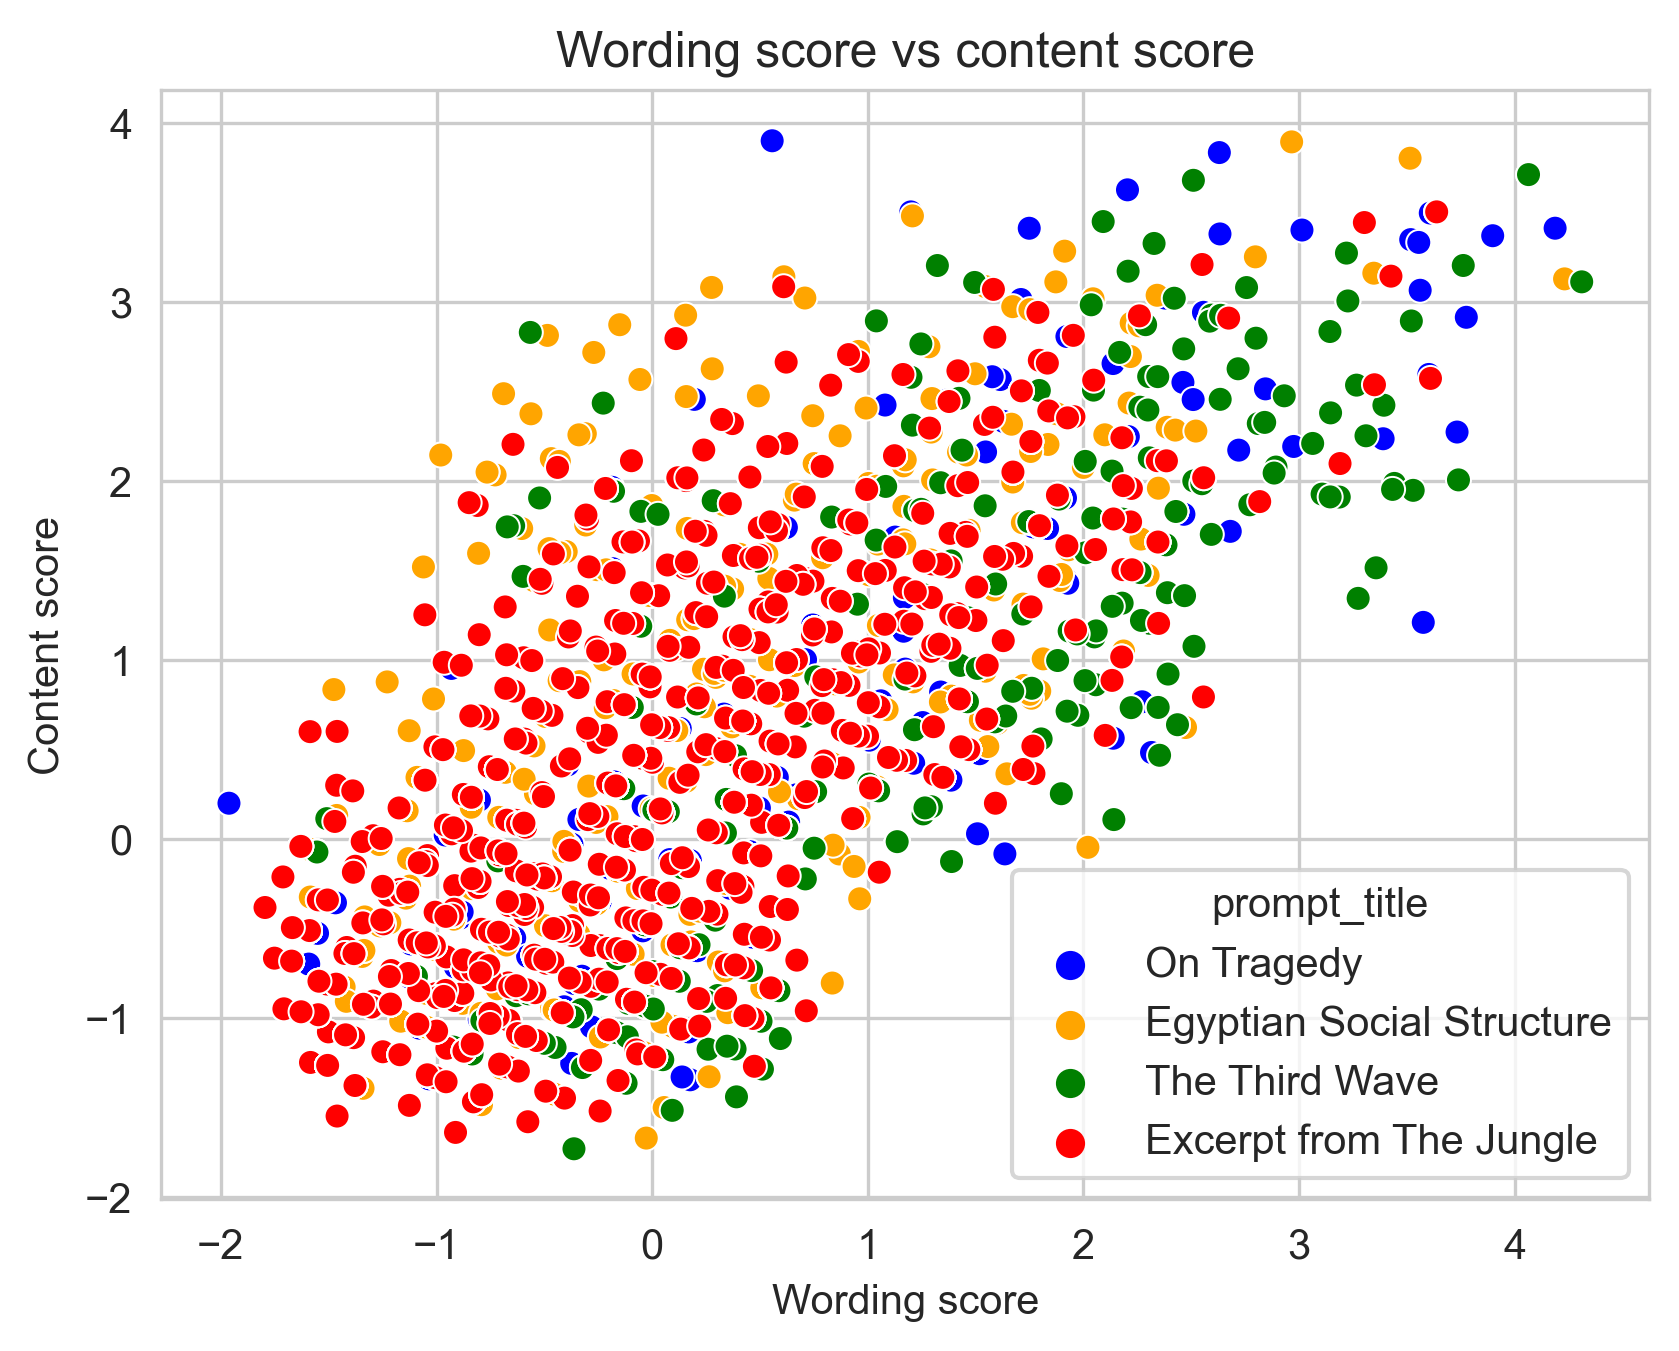
\includegraphics[width=80mm,scale=0.75]{img/wording_content_correlation.png}
\end{center}
\caption[Correlation between Wording and Content scores]{A weak correlation between content and wording scores indicating a small amount of influence between both.}
\label{fig:correlation-con-wor}
\end{figure}
